\section{Week 1 - Introduction and NLP}
\subsection{Introduction}
\subsubsection{What is AI?}
A broad concept with different interpretations.
In this class: Where a computer \textbf{learns from data}.
Often called \textbf{statistical machine learning.}\\
Ultimate research goal: AGI (artificial general intelligence).
a hypothetical computer program that can perform intellectual tasks as well as, or better than, a human.

\subsubsection{How to tell if a machine is intelligent}
With the \textbf{Turing Test:}\\
If the behaviour is indistinguishable from a human, it is intelligent.
Problems: AI mus learn to lie, If a complex problem is too hard for humans.

\subsubsection{Where to use it}
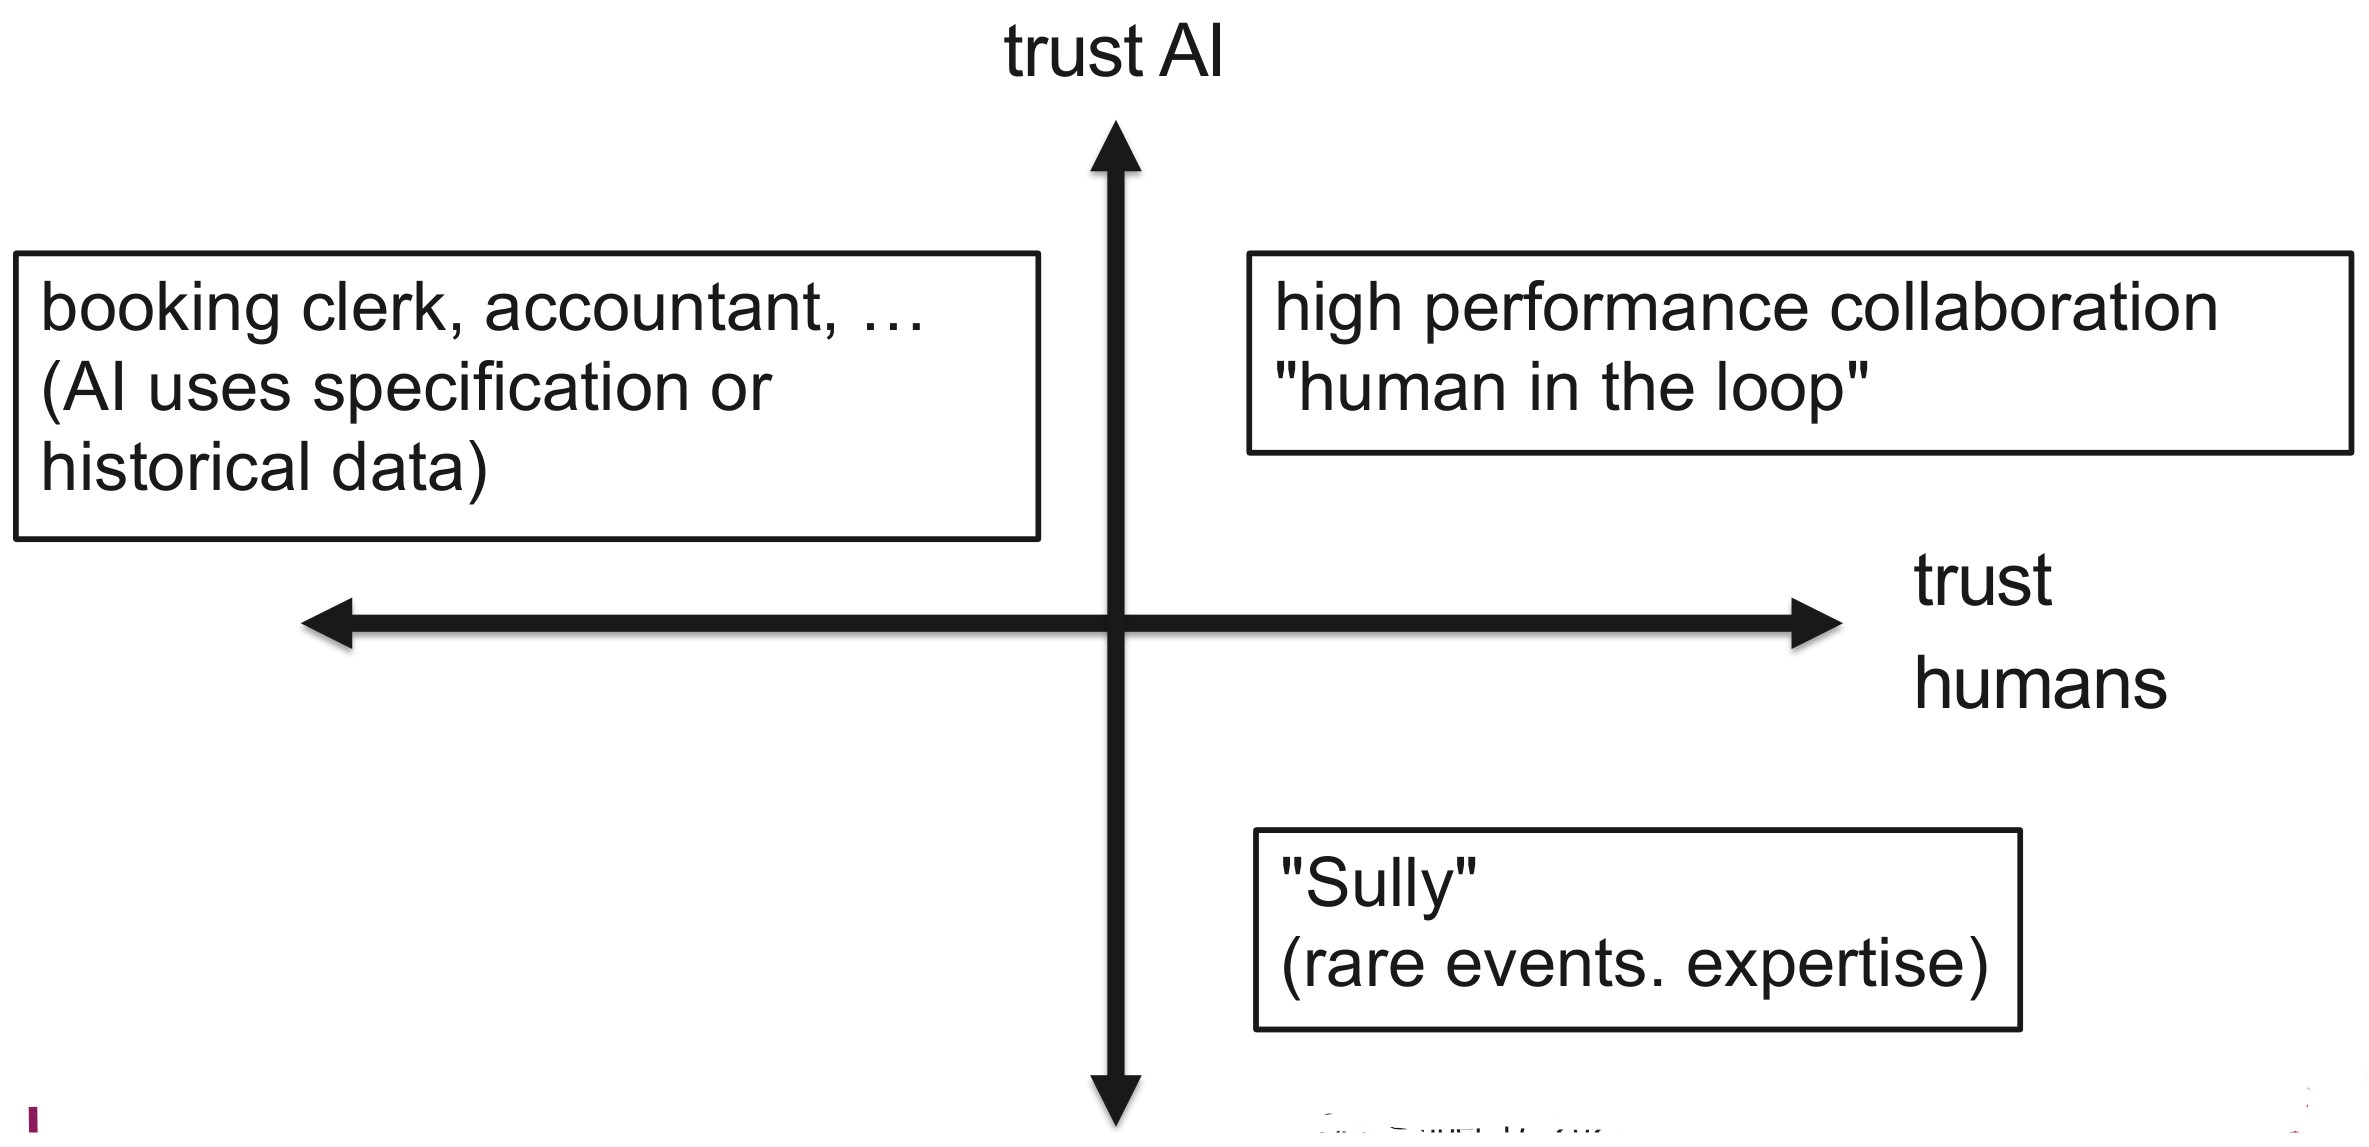
\includegraphics[width=\linewidth]{ai-einsatz.jpg}
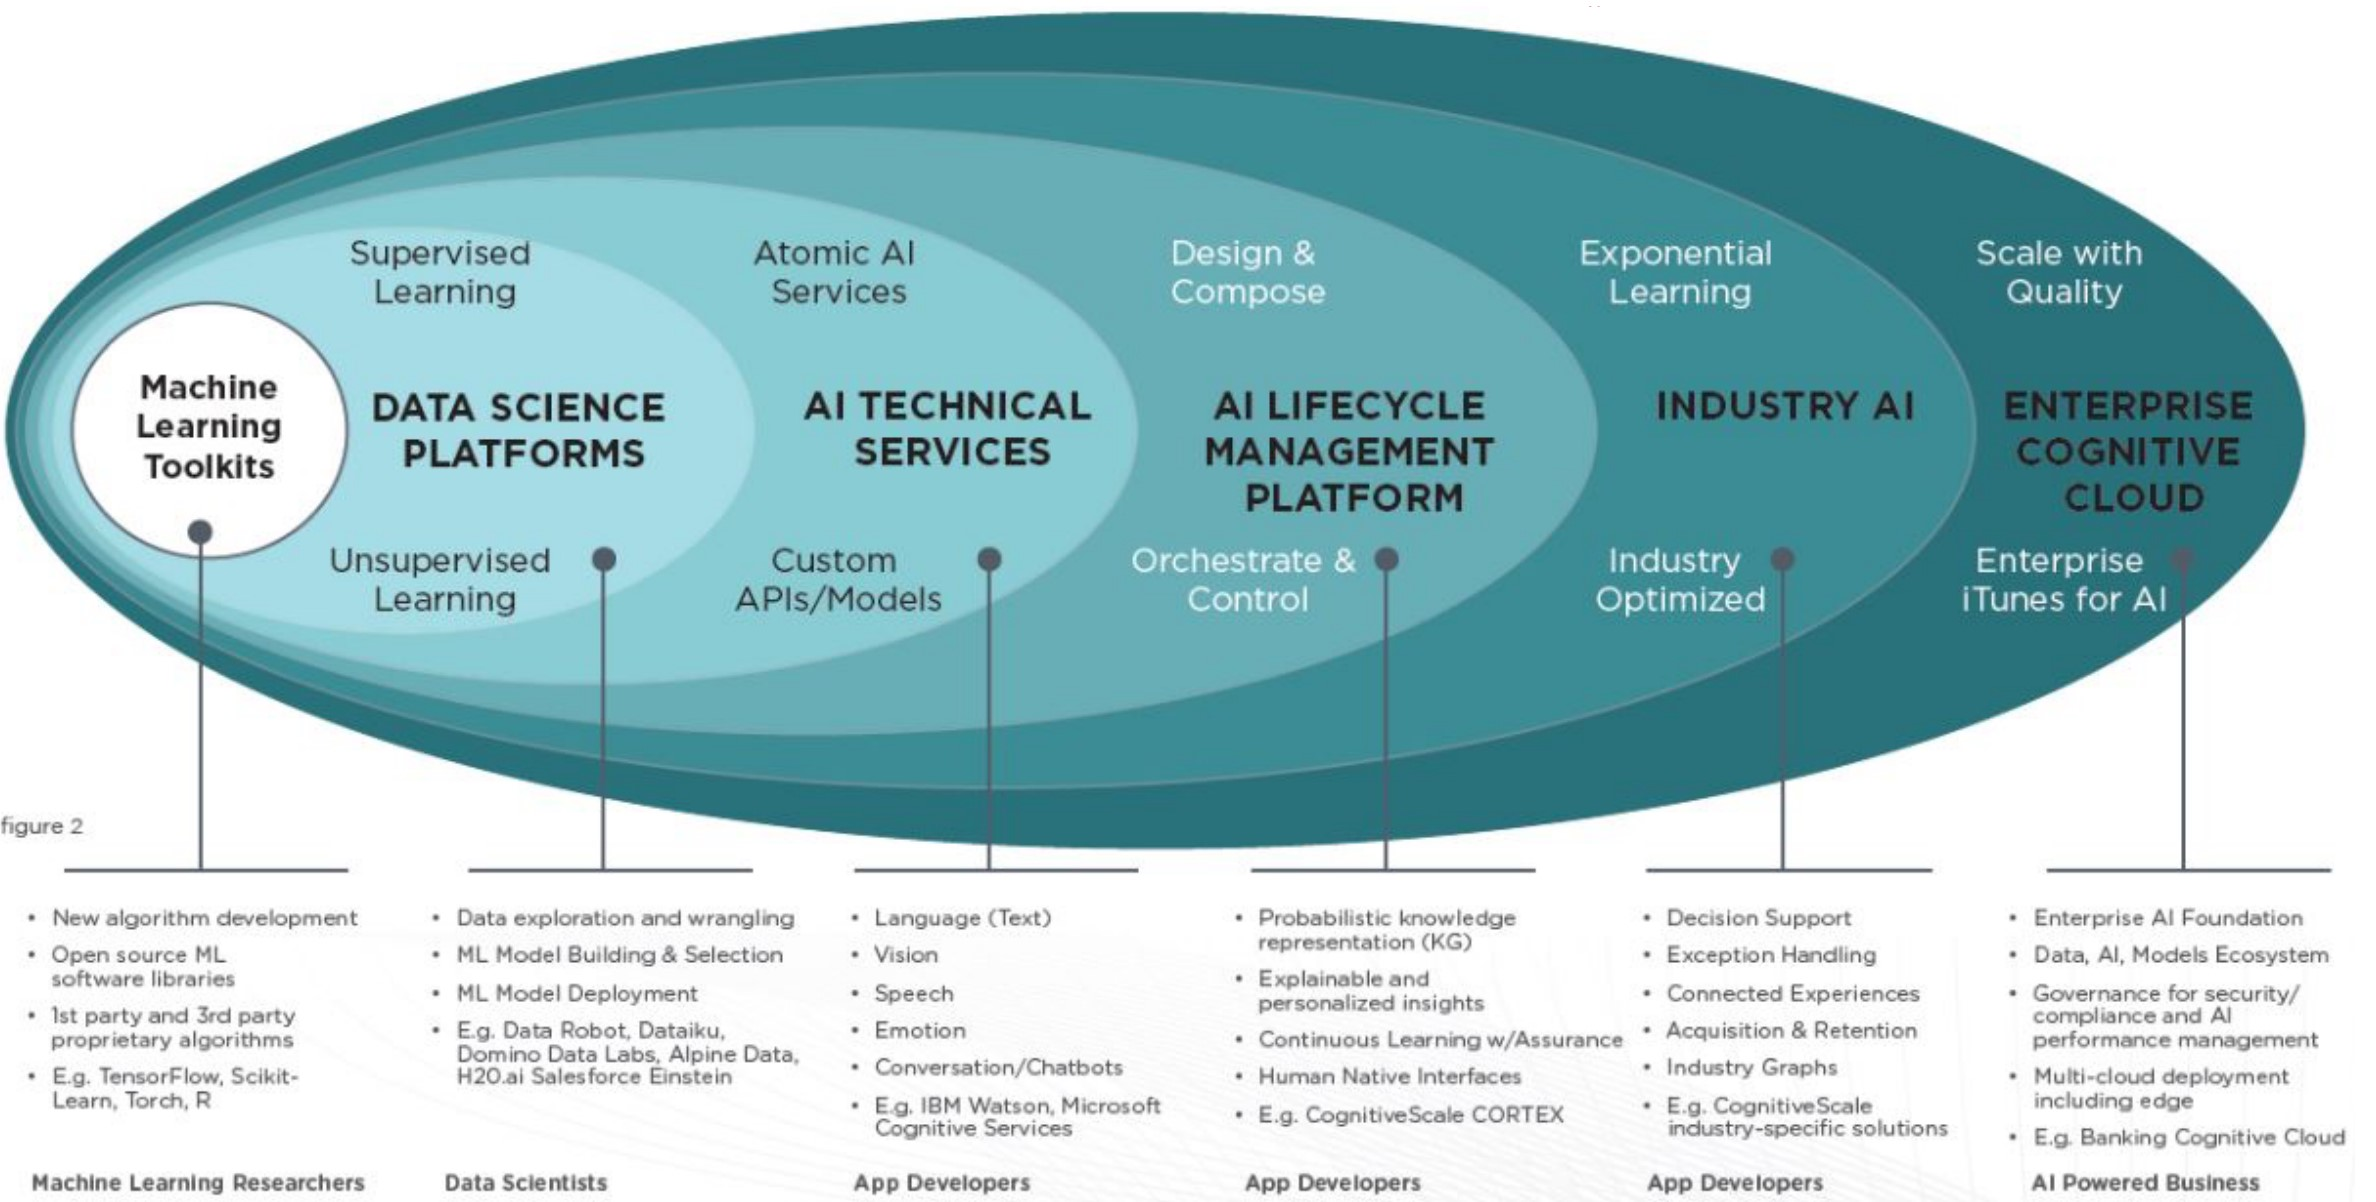
\includegraphics[width=\linewidth]{ai-areas.jpg}

\subsection{NLP (Natural Language Processing)}
NLP is the \textbf{automated processing} of human language.
A Sub-field of AU, aiming to understand and generate language.
Long research history, took-off recently.
Still difficult, but Big-Business.
\subsection{Dialogflow}
\subsubsection{Intents}
What does the user want?
Give example sentences and Dialogflow will generate new sentences to match intent.

\subsubsection{Entities}
Extract information from sentence.
Assign words to entities (variables).
Again, define examples and dialogflow learns new words.

\subsubsection{Dialog Control}
\textbf{Linear:} Collect all Information, for e.g. booking an appointment
\textbf{Non-Linear:} More a real conversation with dependend answers based on changes in context.
Context can be set as Input and Ouput.